\documentclass[../../master.tex]{subfiles}
\usetikzlibrary{rulercompass}

\begin{document}
\section{Geometric impossibilities}

% Problem 3.1
\begin{problem}
    Prove that if $A, B$ are constructible, then the midpoint of the segment $AB$ is also constructible.
    Prove that if two lines $\ell_1, \ell_2$ are constructible and not parallel, then the two lines bisecting the angles formed by $\ell_1$ and $\ell_2$ are also constructible.
\end{problem}

\begin{solution}
    To construct the midpoint of $AB$, draw two circles of radius at least half the length of the segment $AB$ (I think you can just use the radius of the entire line segment): one which is centered at $A$ and one which is centered at $B$.
    These circles should intersect in two places; draw the line connecting them.
    This line will intersect the segment $AB$, and the point at which they intersect is the midpoint of $AB$.

    To construct an angle bisector, consider the angle $\angle AOB$.
    Draw a circle centered at $A$ which intersects both $\ell_1$ and $\ell_2$ at, say, $C$ and $D$.
    Then draw two circles with $C$ and $D$ as centers. 
    These circles should intersect at one point in the region bounded by $\ell_1$ and $\ell_2$, say $E$.
    Finally, draw the line containing both $O$ and $E$.
    This line bisects the angle formed by $\ell_1$ and $\ell_2$.
\end{solution}

% Problem 3.2
\begin{problem}
    Prove that if $a, b$ are constructible numbers, then so is $a - b$.
\end{problem}

\begin{solution}
    First note that $a + b$ is constructible: draw a line through $a$ and $b$ and draw the circle centered at $b$ with radius $a$.
    This circle intersects the line at one other point, which is $a + b$.
    Now note that if $b$ is constructible, $-b$ is also constructible (by the above construction with the circle centered at the origin).
    Since $a$ and $-b$ are constructible, so is $a + (-b) = a - b$.
\end{solution}

% Problem 3.3
\begin{problem}
    Find an explicit straightedge-and-compass construction for the product of two real numbers.
\end{problem}

\begin{solution}
    Given (constructible) $a, b \in \mathbb{R}$, we have explicit constructions for $a$ and $\frac{1}{b}$.
    Then we may construct $a / (1/b) = ab$.
    Note that the below construction does not illustrate this so you should go back and fix it.
    
    \begin{center}
        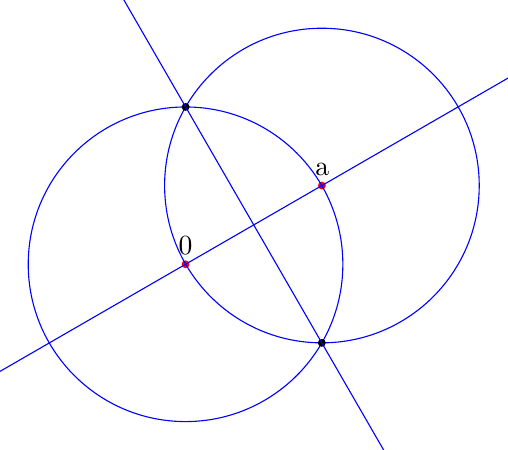
\begin{tikzpicture}[stop jumping, constrain] 
            \path (0, 0) node[name=0, ruler compass/point=red, label={0}];
            \path (0) ++(30:2) node[ruler compass/point=red, label={a}];
            \ruler{0}{a}
            \compass{a}{0}
            \compass{0}{a}
            \point{c0a}{ca0}{1}
            \point{c0a}{ca0}{2}
            \ruler{b}{c}
        \end{tikzpicture}
    \end{center}
\end{solution}

% Problem 3.4
\begin{problem}
    Show how to square a \textit{triangle} by straightedge and compass.
\end{problem}

\begin{solution}
    To do.
\end{solution}
\end{document}
